\chapter{Représentation d'une expression arithmétique en arbre binaire}

\section{Description de l'objectif de l'algorithme}
Une expression arithmétique est une succession de caractères mathématiques notamment des nombres, des opérateurs mathématiques (+ addition, - soustraction, * multiplication, / division et * modulo) et des symboles impropres pour indiquer la priorité( ( ) les parenthèses).
Il faut noter cependant que les opérateurs mathématiques ne possèdent pas tous la même priorité; La multiplication et la division sont plus prioritaires que l'addition et la soustraction.
Dans le cas où la priorité de deux opérateurs est la même, celui le plus à gauche dans l'expression arithmétique devient plus prioritaire que celui à droite.
En considérant ces contraintes, une des représentations les plus adaptées pour décrire une expression arithmétique est l'arbre binaire.
\par
Un arbre binaire est une structure de données complexe, il est caractérisé par un élément racine qui contient à son tour un chemin vers un ou deux autres éléments appelés fils droit et fils gauche. Chaque élément intermédiaire de l'arbre par la suite a la même structure que la racine, jusqu'à arriver aux éléments terminaux qui ne possèdent pas de fils et qu'on nomme les feuilles de l'arbre.
\par
Nous pouvons alors par extrapolation représenter chaque opération arithmétique par un élément de l'arbre, telle que l'élément de l'arbre contient l'opérateur, et les deux opérandes sont contenus dans les deux fils de l'élément.
Pour qu'un arbre binaire puisse représenter la structure d'une expression arithmétique correctement, ce dernier doit respecter l'ordre et la priorité des opérations. Les opérations les moins prioritaires sont en haut de l'arbre car elles dépendent du résultat des opérations plus prioritaires qui elles, sont plus bas dans l'arbre binaire (voir Figure \ref{fig:exp_arbre}).

\begin{figure}[H]
    \centering
        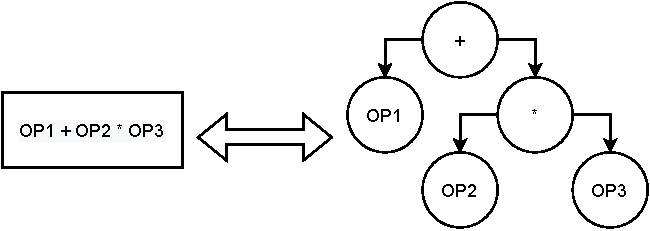
\includegraphics[scale=1.0]{./ressources/expression_to_tree.pdf}
        \caption{Représentation d'une expression arithmétique en arbre binaire}
    \label{fig:exp_arbre}
\end{figure}

\section{Fonctionnement de l'algorithme}
Le passage de l'expression arithmétique en arbre binaire passe par 2 étapes de traduction: l'analyse lexicale et puis la traduction dirigée par la syntaxe (voir Figure \ref{fig:etapes_trad}). L'expression arithmétique est d'abord lue du clavier sous forme de chaîne de caractères. Puis, un vecteur d'entités lexicales est généré à partir de cette chaîne. Enfin, on génère un arbre binaire à partir du vecteur d'entités lexicales.

\begin{figure}[H]
    \centering
        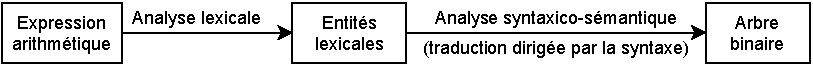
\includegraphics[scale=1.0]{./ressources/translation_steps.pdf}
        \caption{Les étapes de la traduction}
    \label{fig:etapes_trad}
\end{figure}
\par
Les structures de données utilisées dans les algorithmes qui vont suivre sont les suivantes :
\begin{description}
    \item[entité] : représente une entité lexicale et contient les champs type de l'entité et la valeur.     
    \item[noeud] : représente un élément d'un arbre et contient une valeur et des pointeurs vers les fils droit et gauche du noeud.
    \item[arbre] : représente un arbre binaire et contient un pointeur vers la racine de l'arbre.
\end{description}

\subsection{Analyse lexicale}
Dans cette partie, on extrait les entités lexicales de la chaîne de caractères contenant l'expression arithmétique.
On parcourt la chaîne de caractères depuis le début, et on génère les entités lexicales selon les caractères lus.

\begin{algorithm}[H]
    \SetAlgoLined
    \KwData{expression : chaîne de caractères}
    \KwResult{entites : vecteur d'entités}
    \textbf{Variables :}\\
    e : entité\;
    i, j : entier\;
    \Begin{
        Initialiser le vecteur entites à vide\;
        \For{$i \leftarrow 1$\KwTo$expression.taille()$}{
            \uIf{expression[i] est un opérateur}{
                \tcp{Reconnaitre un opérateur}
                e.type$\leftarrow$opérateur\;
                e.operation$\leftarrow$type\_opération\;
                entites.ajouter(e)\;
            }
            \uElseIf{expression[i] est une parenthèse}{
                \tcp{Reconnaitre une parenthèse}
                e.type$\leftarrow$parenthèse\;
                e.parenthèse$\leftarrow$type\_parenthèse\;
                entites.ajouter(e)\;
            }
            \uElseIf{expression[i] est un chiffre ou un point}{
                \tcp{Reconnaitre un nombre}
                j$\leftarrow$1\; 
                \lWhile{$i+j \leq expression.taille()$ et expression[i] est un chiffre ou un point}{j$\leftarrow$$j+1$}
                e.type$\leftarrow$nombre\;
                e.nombre$\leftarrow$en\_nombre(expression.sous\_chaine(i, j))\;
                entites.ajouter(e)\;
                i$\leftarrow$$i+j-1$\;
            }
            \Else{
                Lever une exception\tcp*{Erreur lexicale}
            }
        }
    }
    \caption{Analyse lexicale}
\end{algorithm}

\subsection{Analyse syntaxico-sémantique ou traduction dirigée par la syntaxe}
Nous utilisons l'algorithme de descente récursive pour parcourir le vecteur d'entités et générer l'arbre binaire. Dans cet algorithme chaque MGP (membre de gauche de production) est associé à une fonction dans le programme. L'algorithme commence en appelant une première fois l'axiome de la grammaire et se termine une fois que tout le vecteur est parcouru.
\par
La grammaire utilisée est comme suit :
$$ E \rightarrow T + \{ T \}^* | T - \{ T \}^* $$
$$ T \rightarrow F * \{ F \}^* | F / \{ F \}^* $$
$$ F \rightarrow nb | ( E ) | + F | - F $$

\begin{algorithm}[H]
    \SetAlgoLined
    \KwData{expression : chaîne de caractères}
    \KwResult{entites : vecteur d'entités}
    \textbf{Variables :}\\
    tc : entier\;
    bt : arbre\;
    \Begin{
        ct$\leftarrow$0\;
        \lIf{$tc = entites.taille()$}{Lever une exception\tcp*[f]{Expression vide}}
        bt$\leftarrow$e(entites, tc)\tcp*{Appel de la fonction e}
        \KwRet{bt};
    }
    \caption{Descente récursive}
\end{algorithm}

\par
Cette fonction $e$ traite les opérations d'addition et de soustraction qui sont moins prioritaires, et génère les noeuds correspondants. Le traitement des autres opérations est délégué à la fonction $t$ qui va terminer son exécution avant la fonction $e$; c-à-d. que les noeuds générés par les opérations plus prioritaires seront retournés à la fonction $e$ qui va les ajouter dans les niveaux plus bas.\\
\begin{function}[H]
    \textbf{Variable :}\\
    bt, rt, lt : arbre\;
    e : entité\;
    \Begin{
        bt$\leftarrow$t(entites, tc)\tcp*{Appel de la fonction t}
        \While{$tc \leq entites.taille()$ et entites[tc] est un opérateur d'addition ou de soustraction}{
            e$\leftarrow$entites[tc]\;
            lt$\leftarrow$bt\;
            tc$\leftarrow$tc + 1\;
            \lIf{$tc > entites.taille()$}{Lever une exception\tcp*[f]{Erreur syntaxique}}
            rt$\leftarrow$t(entites, tc)\tcp*{Appel de la fonction t}
            bt.racine$\leftarrow$e\;
            bt.fils\_gauche$\leftarrow$lt\;
            bt.fils\_droit$\leftarrow$rt\;
        }
        \KwRet{bt}\;
    }
    \caption{e(entites : vecteur d'entités, Entrée/Sortie tc : entier) : arbre}
\end{function}

\par
Cette fonction $t$ traite les opérations de multiplication, de division et de modulo. Elle utilise la fonction $f$ pour générer les noeuds des nombres et des sous-expressions plus prioritaires comme les parenthèses.\\
\begin{function}[H]
    \textbf{Variable :}\\
    bt, rt, lt : arbre\;
    e : entité\;
    \Begin{
        bt$\leftarrow$f(entites, tc)\tcp*{Appel de la fonction f}
        \While{$tc \leq entites.taille()$ et entites[tc] est un opérateur de multiplication ou de division ou de modulo}{
            e$\leftarrow$entites[tc]\;
            lt$\leftarrow$bt\;
            tc$\leftarrow$tc + 1\;
            \lIf{$tc > entites.taille()$}{Lever une exception\tcp*[f]{Erreur syntaxique}}
            rt$\leftarrow$f(entites, tc)\tcp*{Appel de la fonction f}
            bt.racine$\leftarrow$e\;
            bt.fils\_gauche$\leftarrow$lt\;
            bt.fils\_droit$\leftarrow$rt\;
        }
        \KwRet{bt}\;
    }
    \caption{t(entites : vecteur d'entités, Entrée/Sortie tc : entier) : arbre}
\end{function}

\par
Cette fonction $f$ génère les noeuds des nombres et des opérateurs unaires, elle repasse le contrôle à la fonction $e$ en cas d'utilisation de parenthèses pour traiter la sous-expression contenue dedans.\\
\begin{function}[H]
    \textbf{Variable :}\\
    bt, rt, lt : arbre\;
    e, gauche, droit : entité\;
    \Begin{
        \uIf{entites[tc] est une parenthèse ouvrante}{
            tc$\leftarrow$tc + 1\;
            \lIf{$tc > entites.taille()$}{Lever une exception\tcp*[f]{Erreur syntaxique}}
            bt$\leftarrow$e(entites, tc)\tcp*{Appel de la fonction e}
            \uIf{$tc \leq entites.taille()$ et entites[tc] est une parenthèse fermante}{
                tc$\leftarrow$tc + 1\;
            }
            \Else{
                Lever une exception\tcp*[f]{Erreur Syntaxique}
            }
        }
        \uElseIf{entites[tc] est un opérateur d'addition ou de soustraction}{
            \tcp{Cas d'un opérateur unaire}
            e$\leftarrow$entites[ct]\;
            gauche.type$\leftarrow$type\_nombre\;
            gauche.nombre$\leftarrow$0\;
            tc$\leftarrow$tc + 1\;
            \lIf{$tc > entites.taille()$}{Lever une exception\tcp*[f]{Erreur syntaxique}}
            rt$\leftarrow$f(entites, tc)\tcp*{Appel de la fonction f}
            lt.racine$\leftarrow$gauche\;
            bt.racine$\leftarrow$e\;
            bt.fils\_gauche$\leftarrow$lt\;
            bt.fils\_droit$\leftarrow$rt\;
        }\Else{
            \tcp{Cas d'un nombre (feuille de l'arbre)}
            e$\leftarrow$entites[tc]\;
            bt.racine$\leftarrow$e\;
            tc$\leftarrow$tc + 1\;
        }
        \KwRet{bt}\;
    }
    \caption{f(entites : vecteur d'entités, Entrée/Sortie tc : entier) : arbre}
\end{function}

\section{Calcul de complexité}
\subsection{Complexité temporelle}
La complexité de l'analyse lexicale est toujours égale à la longueur de la chaîne dans tous les cas c-à-d. : $\mathcal{O}(n)$ tel que $n$ est la longueur de l'expression en de caractères.
\par
La complexité de l'analyse syntaxique est quant à elle égale à la longueur du vecteur d'entités lexicales, car il est parcouru une seule fois, c-à-d. : $\mathcal{O}(n')$ tel que $n'$ est la longueur du vecteur d'entités.
\par
La complexité temporelle de l'algorithme devient alors : $\mathcal{O}(n + n')$. Sachant que $n > n'$ (le nombre de caractères est supérieur au nombre d'opérandes) on peut remplacer $n'$ par $n$, et la formule devient : $\mathcal{O}(n)$ qui est une complexité linéraire.

Le tableau suivant représente les temps d'exécution théorique en nanoseconde de l'algorithme selon la variation de la taille de l'expression:

\small
\begin{center}
\begin{tabular}{| c | c | c | c | c | c | c | c | c | c | c | c | c |}
    \hline
    N & 10 & 50 & 100 & 500 & 1000 & 5000 & 10000 & 100000 & 1000000 & 10000000 \\
    \hline
    t(ns) & 10 & 50 & 100 & 500 & 1000 & 5000 & 10000 & 100000 & 1000000 & 10000000 \\
    \hline
\end{tabular}  
\end{center}

La figure suivante (voir Figure \ref{fig:temps_exec_th_algo2}) représente l'évolution du temps d'exécution théorique selon la longueur de l'expression.

\begin{figure}[H]
    \centering
        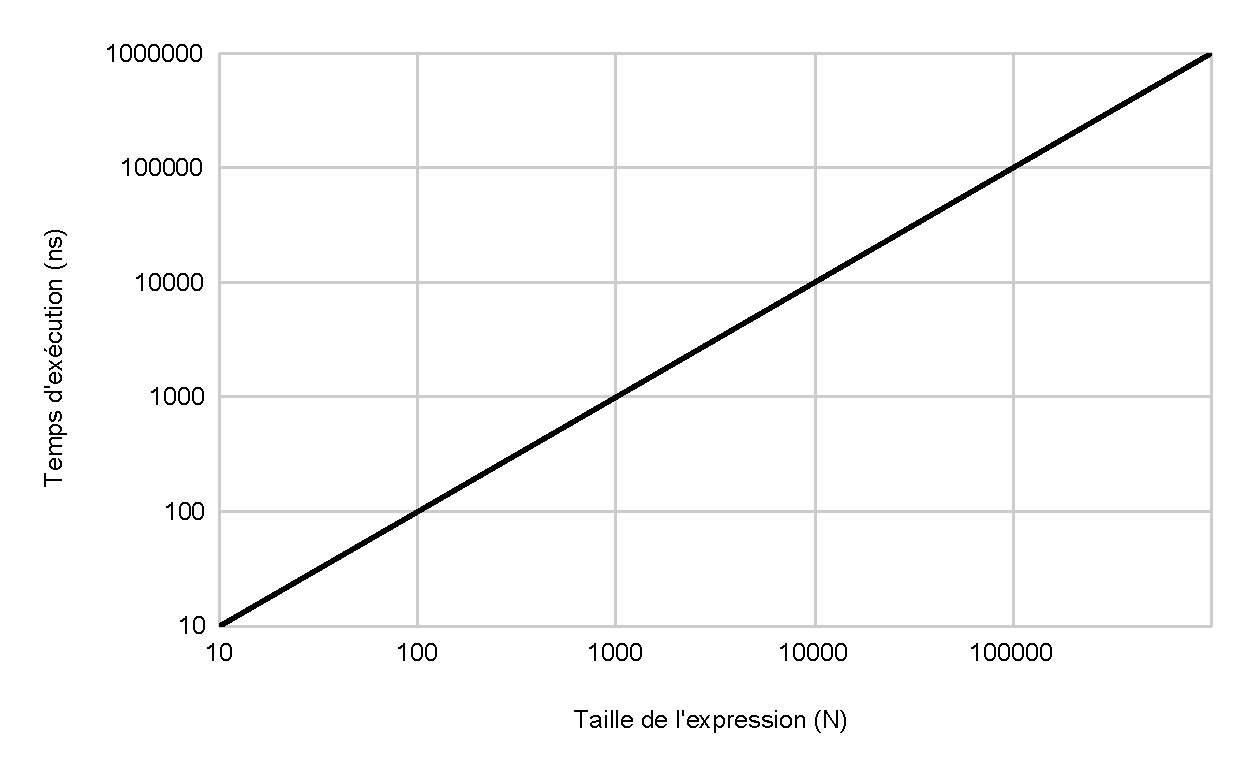
\includegraphics[scale=0.5]{./ressources/temps_execution_th_algo2.pdf}
        \caption{Temps d'exécution théorique de l'algorithme de représentation d'expression arithmétique en arbre binaire}
    \label{fig:temps_exec_th_algo2}
\end{figure} 

Depuis le graphe,  on observe que le temps d'exécution évolue de manière linéaire avec l'évolution de la taille de l'expression.

\subsection{Complexité spatiale}
L'expression arithmétique est d'abord stockée dans une chaîne de caractères de longueur $n$, puis dans un vecteur d'entités de longueur $n'$, puis dans un arbre binaire qui contient lui aussi $n'$ éléments.
\par
Sachant qu'une entité contient le type de l'entité et la valeur en elle-même, cependant la valeur est stockée comme un nombre réel qui prend 8 octets comparé à la représentation en chaîne de caractères où chaque caractère est sous 1 octet.
\par
Donc la taille d'un élément d'une chaîne de caractères est $1$ unité (octet), la taille d'une entité est $9$ unités, et la taille d'un élément d'un arbre est égale à $9 + 4 * 2$ unités (la taille d'un pointeur est égale à $4$ unités) donc $17$ unités.
\par
La complexité spatiale est égale à la somme des trois complexités (taille de la chaîne + taille du vecteur + taille de l'arbre) : $n * 1 + n' * 9 + n' * 17 = n + n' * 26 \approx \mathcal{O}(n + n')$
\par

\section{Expérimentation}
Le tableau suivant représente les temps d'exécution en nanoseconde de l'algorithme selon la variation de la taille de l'expression arithmétique.\\
\small
\begin{tabular}{| c | c | c | c | c | c | c | c | c | c | c | c |}
    \hline
    N &  10 & 50 & 100 & 500 & 1000 & 5000 & 10000 & 100000 & 1000000 \\
    \hline
    t1(ns) & 177584 & 437769 & 381575 & 418252 & 686466 & 3111420 & 6786260 & 60986100 & 642610000 \\
    \hline
    t2(ns) & 101653 & 193648 & 339100 & 354777 & 2322770 & 3307840 & 20424500 & 59967200 & 639145000 \\
    \hline
    t3(ns) & 31972 & 47574 & 216601 & 354751 & 2115200 & 3375350 & 7450650 & 60956700 & 639422000 \\
    \hline
    t4(ns) & 100708 & 149167 & 259485 & 337421 & 820084 & 3283810 & 19698800 & 61631500 & 641354000 \\
    \hline
    t5(ns) & 24343 & 140434 & 95821 & 345987 & 683119 & 5158840 & 7575520 & 61750100 & 640897000 \\
    \hline
    t6(ns) & 30901 & 161277 & 337395 & 807634 & 671850 & 3292160 & 21818400 & 61473700 & 641686000 \\
    \hline
    t7(ns) & 52941 & 140159 & 288308 & 329206 & 693785 & 4360970 & 8418610 & 60870500 & 667895000 \\
    \hline
    t8(ns) & 69185 & 163825 & 242197 & 520649 & 2050330 & 5460620 & 22419800 & 63008000 & 639987000 \\
    \hline
    t9(ns) & 69510 & 97011 & 93270 & 356979 & 692529 & 5279490 & 6420450 & 61725500 & 640873000 \\
    \hline
    t10(ns) & 83819 & 142928 & 92484 & 1071680 & 803473 & 13108600 & 6558390 & 60088300 & 639895000 \\
    \hline
    Moyenne(ns) & 74262 & 167379 & 234624 & 489734 & 1153961 & 4973910 & 12757138 & 61245760 & 643376400 \\
    \hline
\end{tabular}
\normalsize
\par
La figure suivante (voir Figure \ref{fig:temps_exec_algo2}) représente l'évolution du temps d'exécution selon la longueur de l'expression arithmétique.

\begin{figure}[H]
    \centering
        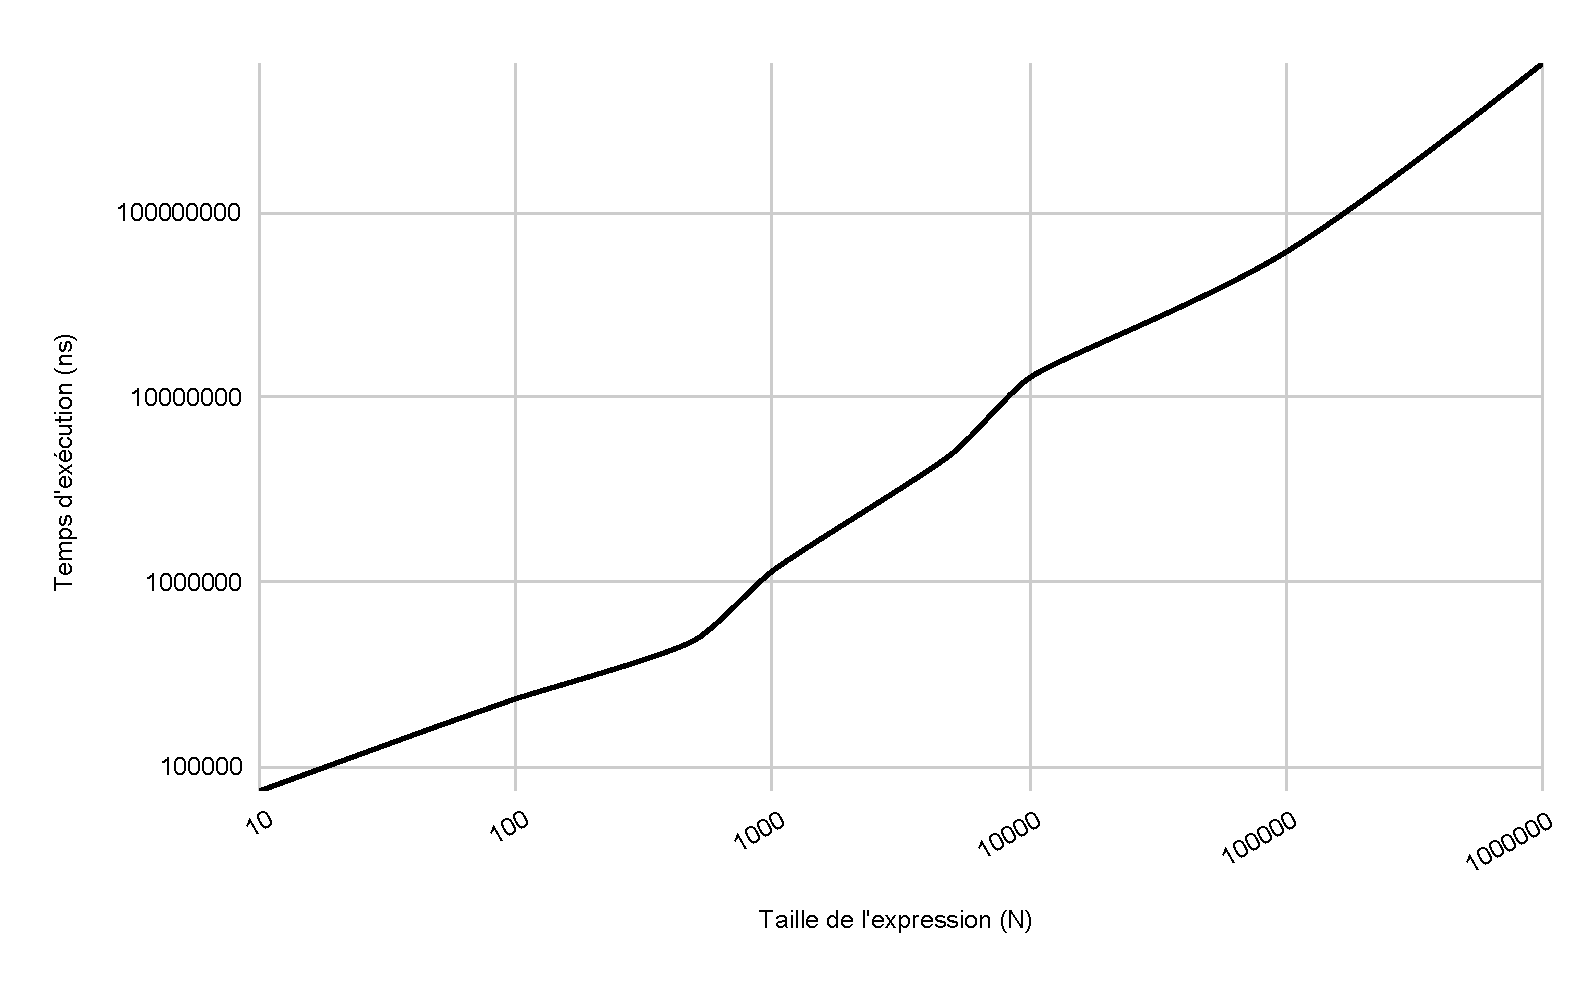
\includegraphics[scale=0.5]{./ressources/temps_execution_algo2.pdf}
        \caption{Temps d'exécution du programme selon la longueur de l'expression}
    \label{fig:temps_exec_algo2}
\end{figure}
\par
Depuis le graphe, la courbe est sous forme d'une droite, on observe que le temps d'exécution évolue de manière linéaire avec l'augmentation de la taille du problème, ce qui correspond bien à la complexité théorique calculée auparavant. 

\section{Conclusion}
L'algorithme de la descente récursive propose une complexité optimale pour la représentation de l'expression arithmétique en arbre binaire, égale à la longueur de l'expression arithmétique, car il parcourt l'expression un nombre minimal de fois (une seule fois). Nous avons bien vu pendant les expériences que l'évolution du temps d'exécution d'une telle complexité est relativement contrôlée et suit une courbe droite et linéaire.
